\documentclass{thesisclass}
% Based on thesisclass.cls of Timo Rohrberg, 2009
% ----------------------------------------------------------------
% Thesis - Main document
% ----------------------------------------------------------------
% No empty in-between chapters, remove this line if desired for double-page printing
%\let\cleardoublepage\clearpage


\newcommand{\til}{{\raise.17ex\hbox{$\scriptstyle\mathtt{\sim}$}}}

\usepackage{mathtools}
\usepackage{pdfcomment}
\usetikzlibrary{decorations.pathreplacing,angles, quotes, calligraphy, fit, shadings}
\usepackage{tikzpagenodes}

\newcommand{\bigO}{\mathcal{O}}

\usepackage{lineno}
\makeatletter
\def\makeLineNumberLeft{%
  \linenumberfont\llap{\hb@xt@\linenumberwidth{\LineNumber\hss}\hskip\linenumbersep}% left line number
  \hskip\columnwidth% skip over column of text
  \rlap{\hskip\linenumbersep\hb@xt@\linenumberwidth{\hss\LineNumber}}\hss}% right line number
\leftlinenumbers% Re-issue [left] option
\makeatother

%\linenumbers

\usepackage{xargs}                      % Use more than one optional parameter in a new commands
%\usepackage[pdftex,dvipsnames]{xcolor}  % Coloured text etc.

\usepackage[colorinlistoftodos,prependcaption,textsize=tiny]{todonotes}
\newcommandx{\unsure}[2][1=]{\todo[linecolor=red,backgroundcolor=red!25,bordercolor=red,#1]{#2}}
\newcommandx{\change}[2][1=]{\todo[linecolor=blue,backgroundcolor=blue!25,bordercolor=blue,#1]{#2}}
\newcommandx{\info}[2][1=]{\todo[linecolor=OliveGreen,backgroundcolor=OliveGreen!25,bordercolor=OliveGreen,#1]{#2}}
\newcommandx{\improvement}[2][1=]{\todo[linecolor=Plum,backgroundcolor=Plum!25,bordercolor=Plum,#1]{#2}}
\newcommandx{\thiswillnotshow}[2][1=]{\todo[disable,#1]{#2}}

\setlength{\marginparwidth}{20mm}

\usepackage{booktabs}
\newcommand{\ra}[1]{\renewcommand{\arraystretch}{#1}}


\usepackage{subcaption}
\usetikzlibrary[spy,calc]

\usepackage{pgf}
\usepackage{acronym}

\usepackage{footnote}
\usepackage{svg}

\makesavenoteenv{tabular*}
\DeclareMathOperator*{\argmax}{arg\,max}
\DeclareMathOperator*{\argmin}{arg\,min}

\DeclarePairedDelimiter\abs{\lvert}{\rvert}%
\DeclarePairedDelimiter\norm{\lVert}{\rVert}%

\usepackage{calc}

\usepackage[export]{adjustbox}

\usepackage{algorithm}
\usepackage[noend]{algpseudocode}

\makeatletter
\def\BState{\State\hskip-\ALG@thistlm}
\makeatother

\pdfinclusioncopyfonts=1
\usepackage[activate={true,nocompatibility}]{microtype}

\newcommand{\dif}{\mathop{}\!\mathrm{d}}

\usepackage{amssymb}
\usepackage{placeins}

\newcommand\blfootnote[1]{%
  \begingroup
  \renewcommand\thefootnote{}\footnote{#1}%
  \addtocounter{footnote}{-1}%
  \endgroup
}

%\usepackage[toc,page]{appendix}


%% -------------------------------
%% |  Information for PDF file   |
%% -------------------------------
\hypersetup{
 pdfauthor={Andreas Mikolajewski},
 pdftitle={Efficient datastructures and sampling of many light sources for Next Event Estimation},
 pdfsubject={Photon-based Next Event Estimation},
 pdfkeywords={Computer graphics, photorealism, path tracer, Next Event Estimation, importance sampling}
}


%% ---------------------------------
%% | Information about the thesis  |
%% ---------------------------------

\newcommand{\myname}{Andreas Mikolajewski}
\newcommand{\mytitle}{Efficient datastructures and sampling of many light sources for \\Next Event Estimation}
\newcommand{\myinstitute}{KIT Computer Graphics}

\newcommand{\reviewerone}{Prof. Dr.-Ing. Carsten Dachsbacher}
\newcommand{\reviewertwo}{Prof. Dr. Hartmut Prautzsch}
\newcommand{\advisor}{Dr. Johannes Schudeiske (Hanika)}
\newcommand{\advisortwo}{?}

\newcommand{\timestart}{XX. Monat 20XX}
\newcommand{\timeend}{XX. Monat 20XX}
\newcommand{\submissiontime}{DD. MM. 20XX}

%% --------------------------------
%% | Settings for word separation |
%% --------------------------------
% Help for separation:
% In german package the following hints are additionally available:
% "- = Additional separation
% "| = Suppress ligation and possible separation (e.g. Schaf"|fell)
% "~ = Hyphenation without separation (e.g. bergauf und "~ab)
% "= = Hyphenation with separation before and after
% "" = Separation without a hyphenation (e.g. und/""oder)

% Describe separation hints here:
\hyphenation{
% Pro-to-koll-in-stan-zen
% Ma-na-ge-ment  Netz-werk-ele-men-ten
% Netz-werk Netz-werk-re-ser-vie-rung
% Netz-werk-adap-ter Fein-ju-stier-ung
% Da-ten-strom-spe-zi-fi-ka-tion Pa-ket-rumpf
% Kon-troll-in-stanz
}


%% ------------------------
%% |    Including files   |
%% ------------------------
% Only files listed here will be included!
% Useful command for partially translating the document (for bug-fixing e.g.)
\includeonly{
titlepage,
content,
chapters/abstract,
chapters/introduction,
chapters/fundamentals,
chapters/previouswork,
chapters/PNEE,
chapters/implementation,
chapters/evaluation,
chapters/prospect,
chapters/appendix,
acronym
}

\makeatletter

\newrobustcmd*{\parentexttrack}[1]{%
  \begingroup
  \blx@blxinit
  \blx@setsfcodes
  \blx@bibopenparen#1\blx@bibcloseparen
  \endgroup}

\AtEveryCite{%
  \let\parentext=\parentexttrack%
  \let\bibopenparen=\bibopenbracket%
  \let\bibcloseparen=\bibclosebracket}

\makeatother

\addbibresource{thesis.bib}

%%%%%%%%%%%%%%%%%%%%%%%%%%%%%%%%%
%% Here, main documents begins %%
%%%%%%%%%%%%%%%%%%%%%%%%%%%%%%%%%
\begin{document}

\frontmatter
\pagenumbering{roman}
%% titlepage.tex
%%

% coordinates for the bg shape on the titlepage
\newcommand{\diameter}{20}
\newcommand{\xone}{-15}
\newcommand{\xtwo}{160}
\newcommand{\yone}{15}
\newcommand{\ytwo}{-253}

\begin{titlepage}
% bg shape
\begin{tikzpicture}[overlay]
\draw[color=gray]  
 		 (\xone mm, \yone mm)
  -- (\xtwo mm, \yone mm)
 arc (90:0:\diameter pt) 
  -- (\xtwo mm + \diameter pt , \ytwo mm) 
	-- (\xone mm + \diameter pt , \ytwo mm)
 arc (270:180:\diameter pt)
	-- (\xone mm, \yone mm);
\end{tikzpicture}
	\begin{textblock}{10}[0,0](4,2.5)
		
\includegraphics[width=.3\textwidth]{logos/KITLogo_RGB.pdf}
	\end{textblock}
	\changefont{phv}{m}{n}	% helvetica	
	\vspace*{3.5cm}
	\begin{center}
		\Huge{\mytitle}
		\vspace*{2cm}\\
		
		\vspace*{1cm}
		\huge{\myname}\\
		\vspace*{6cm}
		\Large{
			\myinstitute
			\\Master thesis
		}\\
		\vspace*{1cm}
		\Large{\today}
	\end{center}
	\vspace*{1cm}
%\Large{
%\begin{center}
%\begin{tabular}[ht]{l c l}
%  % Gutachter sind die Professoren, die die Arbeit bewerten. 
%  \iflanguage{english}{Reviewer}{Erstgutachter}: & \hfill  & \reviewerone\\
%  \iflanguage{english}{Second reviewer}{Zweitgutachter}: & \hfill  & \reviewertwo\\
%  \iflanguage{english}{Advisor}{Betreuender Mitarbeiter}: & \hfill  & \advisor\\
%  \iflanguage{english}{Second advisor}{Zweiter betreuender Mitarbeiter}: & \hfill  & \advisortwo\\
%  % Der zweite betreuende Mitarbeiter kann weggelassen werden. 
%\end{tabular}
%\end{center}
%}


\vspace{2cm}


\begin{textblock}{10}[0,0](4,16.8)
\tiny{ 
		{KIT -- Universität des Landes Baden-Württemberg und nationales Forschungszentrum der Helmholtz-Gesellschaft}
}
\end{textblock}

\begin{textblock}{10}[0,0](14,16.75)
\large{
	\textbf{www.kit.edu} 
}
\end{textblock}

\end{titlepage}

\blankpage

\chapter*{Abstract}

Modern photorealistic media production faces an increasing number of light sources to produce natural-looking images. A very significant percentage of processing time goes towards casting shadow rays to calculate the direct lighting term with Next Event Estimation. Naively sampling many light sources in a path tracer quickly becomes impractical, as our evaluation shows. We present a novel technique to importance sample many light sources called Photon-based Next Event Estimation (PNEE). In a preprocess,  similar to photon mapping, photons are scattered from all light sources into the scene. These photons are used to build cumulative distribution functions (CDF) that reflect the importance of the light sources to reduce the variance of Monte Carlo Integration. We evaluate several storage options and data structures for efficient lookups within the integrator. We introduce and utilize two novel data structures to store CDFs: sparse CDFs and interpolated CDFs. To mitigate variance edges and artifacts, we present several interpolation and approximation techniques. We evaluate several variants of PNEE against naive NEE as well as PBRTs recent implementation, and demonstrate that even for moderately complex scenes a 50-100x speedup can be achieved.
%% -------------------
%% |   Directories   |
%% -------------------
\listoftodos[Notes]
\tableofcontents
\blankpage


%% -----------------
%% |   Main part   |
%% -----------------
\mainmatter
\pagenumbering{arabic}
%% ==============================
\chapter{Introduction}
\label{ch:Introduction}
%% ==============================

\section{Motivation}

Modern photorealisitic rendering is commonly done by path tracers. With an ever expanding complexity of modelled scenes the presence of many light sources greatly contributes to a natural and appealing image. Path tracers utilize Next Event Estimation to deterministically connect ray intersections (shading points) with light sources. This process is a critical step in modern path tracers and takes up to 50\% of today's rendering time, partially because calculating the visibility term is costly. As sampling all lights quickly becomes too expensive for scenes with more then a few dozen lights, sampling only one or some lights per intersection is a common approach to greatly reduce the rendering time of scenes with a lot of occlusion respectively localized light influences. In an attempt to reduce the variance it is apparent that you want to sample light sources with a higher contribution with a higher probability and try to spare any unnecessary work of sampling occluded light sources. An important aspect is to stay unbiased during this process. We investigate current techniques and propose a new solution to this problem.
%% ==============
\chapter{Fundamentals}
\label{ch:Fundamentals}
%% ==============


%% ==============
\section{Rendering equation}
\subsection{Radiometry}
\subsection{Raytracer}
\subsection{Light Path Expressions}
\subsection{Measurement Contribution Function}


%% ==============
\section{Sampling}

\subsection{Probablity Density Function}

\subsection{Cumulative Distribution Function}

\subsection{Inverse Transform Sampling}

\subsection{Monte Carlo Integration}
\label{sec:MC}

\subsection{Importance Sampling}
\label{sec:IS}

\subsection{Multiple Importance Sampling}

%% ==============
\section{Bidirectional scattering distribution function}
% mainly only for introduction of specular vs diffuse reflections


%% ==============
\section{Light sources}


%% ==============
\section{Path Tracing}
\subsection{Next Event Estimation}



%% ==============
\section{Photon Mapping}

\subsection{Progressive Photon Mapping}

\subsection{Stochastic Progressive Photon Mapping}



%% ==============
\section{Instant Radiosity}

%% ==============
\section{Datastructures}

% Teapot in a stadium ...

\subsection{Bounding Volume Hierarchy}
\subsection{Grid}
\subsection{Octree}
\subsection{k-d Tree}
\subsection{Surface Area Heuristic}

\section{Interpolation}
\subsection{Scattered data}
\subsection{Structured data}
\subsection{Global methods}


%% ==============
\section{Machine Learning}

\subsection{Fuzzy k-means}
\subsection{Agglomerative Hierarchical Clustering}
\subsection{Expectation Maximaization}
\subsection{Transductive Support Vector Machine}
%% ==============
\chapter{Related Work}
\label{ch:Prev}
%% ==============

We already introduced many academic techniques we base our work on in the last section. In this section we further evaluate past and recent work especially on the field of Next Event Estimation and particularly handling many light sources.

\section{Early work}

Early work on this topic from \parencite{Shirley:1996:MCT:226150.226151} introduces the construction of probability density functions (PDF) for simple area light shapes. Sampling within an area light is a problem on it's own, but is well understood for basic shapes. Further, those PDFs can be combined to inherit multiple light sources. \parencite{Shirley:1996:MCT:226150.226151} discuss weighting the sampling probability of the light sources uniformly and energy based which produces reasonable results in simple scenes but quickly breaks down with many light sources and occlusion. They further propose a technique to spatially divide the scene with an octree to account for more localized influences. Still calculations remain based on emitted energy % angle? 
and spatial distance and fail to attribute for any kind of occlusion.

\section{Lightcuts}

\section{Lighttree}

More recent work from \textcite{Estevez} is inspired by lightcuts \parencite{Walter2005LightcutsAS} and proposes the construction of a lighttree. The leafs are light sources which get pooled into clusters by position as well as orientation. Later, to choose a  light source the tree is traversed down until a cluster with a fitting position and normal cone is found. All lights below the found cut are then sampled uniformly or energy based.

\section{Grid caching}

\parencite{Vevoda} propose a technique which utilizes a light tree and cuts as well (\parencite{Walter2005LightcutsAS}). The scene is subdivided into a regular grid where each cell does hold a cut of the light tree. Similar to \parencite{Estevez} this cut can be used to importance sample given light sources. The kicker is that a cut is calculated lazily only when a shading point within an empty cell is rendered. Other shading points within this cell will later reuse the same cut.

\section{Reinforcement learning}

Another recent work from \parencite{DBLP:journals/corr/DahmK17} utilizes machine learning. It more generally learns light transport paths by learning a $\mathcal{Q}$-function with reinforcement learning. The $\mathcal{Q}$-functions are distributed in screen space and form a Voronoi diagram which guides sampling.


\section{Datastructures}

% research on kd-tree acceleration? Or hashed grids and more advanced grids

\section{Outlook}

Similar problems can be found on work about Instant Radiosity \parencite{keller1997instant, Walter2005LightcutsAS, dachsbacher2014scalable}. Due to the large amount of virtual point lights several techniques had been developed to scale sublinearly. We have to consider these techniques with caution, as one of our main goals is to stay unbiased, while most work on Instant Radiosity is dependent on biased approximations.


%% ==============
\chapter{Photon-based Next Event Estimation}
\label{ch:PNEE}
%% ==============

\section{Hashed grid}

\section{k-d Tree}

\section{Photons or CDFs}

\section{Further Optimizations}

\subsection{Interpolating CDFs}

\subsection{Normal culling}

\subsection{Sparse CDFs}

\section{Adaptive Parametrization}

\subsection{Photon Count}


We try to propose a novel approach to find good estimators for importance sampling (especially) for scenes with many localized light sources. In a preprocess all light sources scatter out photons into the scene, similar to photon mapping (\cite{jensen2001realistic}), but no bounces are considered, as we only need direct light paths for our Next Event Estimation estimator. Further, we only consider LD paths, all LS*D paths can be disregarded. Those paths are disregarded by the first condition anyway, but we distinctly point out that refractions of any kind make a photon obsolete for our usecase. We spatially subdivide our scene with a fitting (yet to be determined) datastructure like a grid, octree or kd-tree. 

We consider either storing photons or PDFs as leaf nodes. When storing photons a k-nearest neighbors search is performed. Each photon holds information about which light source it belongs to. It can be considered if storing more information like a direction or energy may be useful. Energy may be useful in a case where photons are not scattered out evenly but with some kind of PDF. Alternatively a search may be limited by spatial dimensions instead of doing a kNN-search. In a well populated scene both approaches should perform similarly. The collected photons are then used to construct a PDF based on the photon counts (and energy), which is used as an estimator. This approach requires to store many photons in a datastructure and a search operation for each shading point. An alternative may be to directly store a PDF for a region. During the preprocess the PDF is directly adjusted whenever a photon lands. Later any shading point only has to determine which cell it belongs to. The PDF is directly accessible. The datastructure should be more lightweight and access is faster, but the tradeoff to storing photons is that we give up accuracy for individual shading points and we may introduce potentially visible edges of variance on the datastructure bounds. Further considerations and ideas for storing and constructing a datastructure may arise from (stochastically) progressive photon mapping (\cite{Hachisuka2008ProgressivePM} \cite{Hachisuka2009StochasticPP}) and similar techniques.

Another potential key factor may be the regulation of the distribution of the photons. A good measure has to be found to determine the number of photons that have to be scattered by any light source. This may simply be a constant. Alternatively, you could measure how much impact the last batch of photons had on the PDFs inside the datastructure. Lastly, a condition for the count of photons in each spatial region may be utilized. More ideas may arise from literature on photon mapping. Further, potentially a technique to scatter photons not uniformly but based on a PDF may be worthwhile, so that thinly populated areas of the scene may be better populated. This is subject of further research and may be out of scope of this work.

We may explore how Multiple Importance Sampling (MIS) might further mature the stability of this technique. As we may have a good estimation how good our estimator will be based on the number of photons of the shading point surroundings, it might be a good idea to offload the sampling importance to a traditional estimator for thinly populated shading points.

The implementation will be based on PBRT (\cite{pbrt}).


%% ==============
\chapter{Implementation}
\label{ch:Implementation}
%% ==============

%% ==============
\section{PBRT}
\subsection{Distribution1D}

\section{k-d tree}

\section{k-means}


%% ==============
\chapter{Evaluation}
\label{ch:Evaluation}
%% ==============
In this chapter we compare all the techniques we implemented with plain uniform and powerbased Next Event Estimation and PBRTs implementation. We try to point out the strength and weaknesses of the techniques for certain kind of scenes and scenarios. In this context we mainly argue about image quality, time and memory. We compare time and momery consumtion based on the Mean Squared Error (MSE) metric from equation~\ref{eq:mse}. Where $Y_i$ is the vector of pixels of length $n$ of our reference image and $\widetilde{Y}_i$ is the vector of pixels of the compared image. 

\begin{align}\label{eq:mse}
\text{MSE} = \frac{1}{n}\sum_{i=1}^{n}\abs{Y_i - \widetilde{Y}_i}^2
\end{align}
\begin{align}\label{eq:rmse}
\text{RMSE} = \sqrt{\text{MSE}}
\end{align}


We compare based on an equal MSE, therefor the MSE is an estimator for our image quality. When we argue about image quality throughout this chapter we rather refer to the perceived image quality\footnote{The MSE in itself has a perception compontent because of the square. The MSE is a very commonly used estimator, nonetheless one could imagine using a metric which does reflect human perception more closely. This usually leads to problems with subjectivity.}, in our case this usually means whether sensible artifacts are present. As all the compared techniques are unbiased, given unlimited time, all of them would converge to the same image. Artifacts are usually areas or edges which will converge very slowly, in practice maybe never. When we say a technique has a bad image quality, we say that artifacts are present. 

\begin{align}\label{eq:sigmaCor}
\sigma \sim \frac{1}{\sqrt{N}}
\end{align}

...

\begin{figure}
\centering
\begin{subfigure}[b]{1\textwidth}
   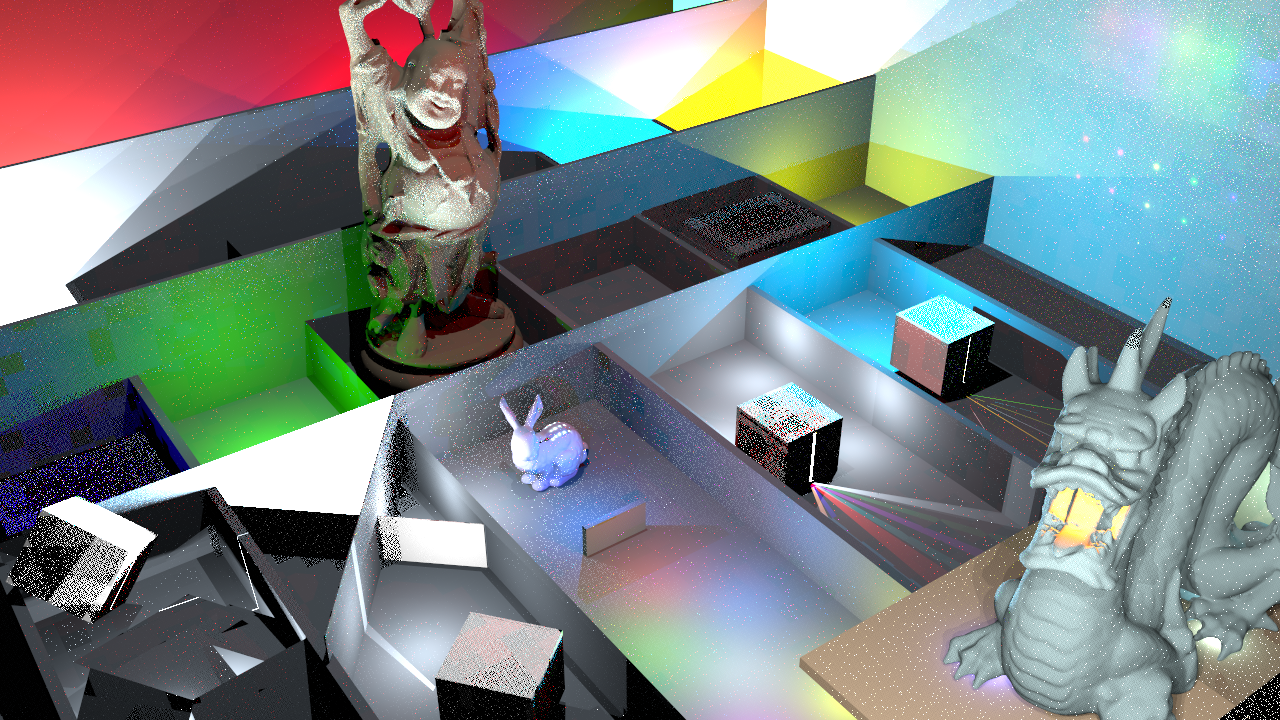
\includegraphics[width=1\linewidth]{figures/examples/StanfordMuseum_pvox_ps512_t503_icdf-0_pc96000k_mc0,1_Vox96_8854.png}
   \caption{Stanford-Museum rendered with 512 samples per pixel with \textit{cdfgrid} and no interpolation.}
   \label{fig:SMnoInt} 
\end{subfigure}

\begin{subfigure}[b]{1\textwidth}
   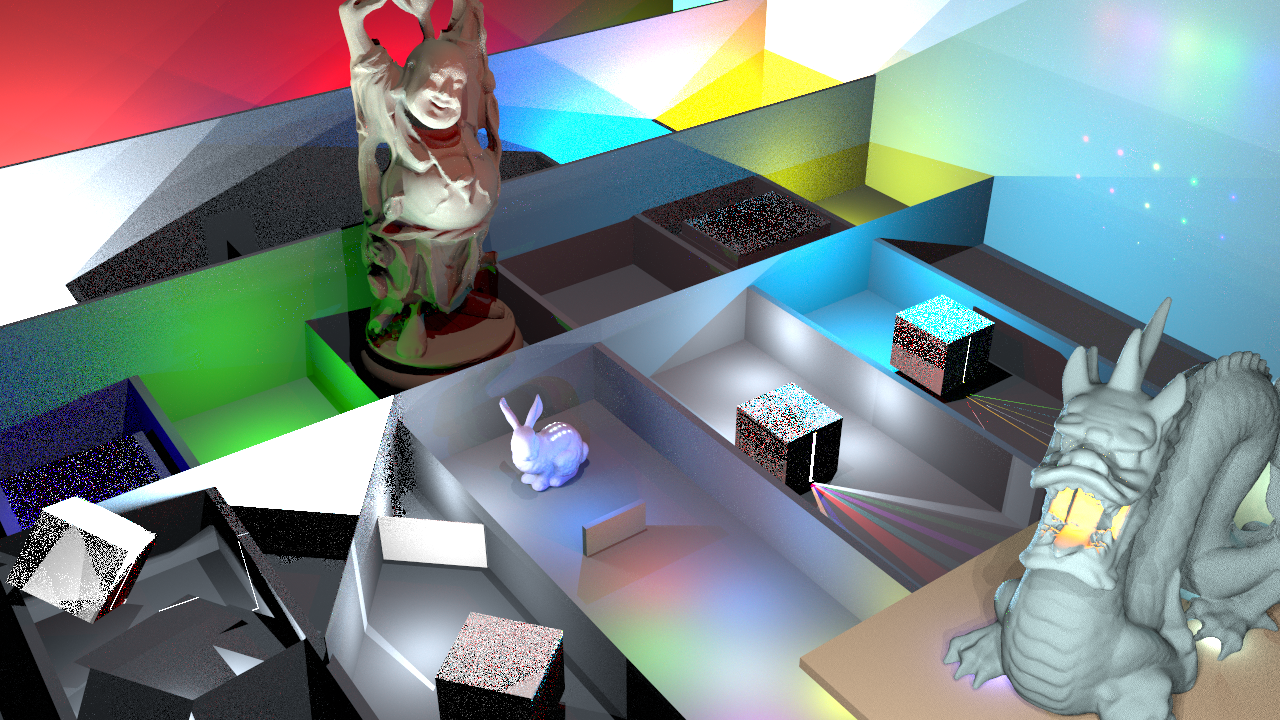
\includegraphics[width=1\linewidth]{figures/examples/StanfordMuseum_pvox_ps512_t723_icdf-1_pc128000k_mc0,1_Vox64_17574.png}
   \caption{Stanford-Museum rendered with 512 samples per pixel with \textit{cdfgrid} and trilinear interpolation.}
   \label{fig:SMInt}
\end{subfigure}

\caption{A visual comparison of no interpolation vs trilinear interpolation. Even though we already have a rather high sample per pixel count, (a) shows many clear variance edges of the underlying grid cells and various artifacts across the scene. Also it is remarkable how many fireflies are visible and how almost none of them are present in (b). It is quite apparent that a human observer would grade the image quality of (b) much higher, but surprisingly the RMSE of (a) is significantly smaller, $39.8$ versus $47.3$. The reason being, that aside of the fireflies and artifacts, the majority of pixels in (a) are less noisy. The difference in noise is less apparent at first, but is well illustrated on the white/gray wall to the left of the Buddah.}
\end{figure}


\section{Setup}

The test machine we use for comparisons is an Intel i7-4790K CPU @ 4GHz, 32 GB RAM, running on Windows 10 64-Bit. Images are produced by PBRT-v3, forked on March 30\footnote{Latest commit before the fork: \url{https://github.com/mmp/pbrt-v3/commit/42c42c194bab970d8adc3f6b5e3afbbc172c3375}}. PNEE techniques are added on top of this fork, the complete implementation can be found at \url{https://github.com/AndiMiko/pbrt-v3}.

\subsection{Problem cases}

We tried to identify problematic light and object constellations, which are causing trouble for various kinds of techniques. The most prominent and comprehensible scenarios are to be covered bellow. 

\begin{description}
    \item[1. High Frequency.] 
    \item[2. Level of Detail.]
    \item[3. High variantion of light power.] 
    \item[4. High number of contributing light sources.]
    \item[5. Non-axis aligned planes.]
    \item[6. Highly occluding planes.]
    \item[7. Tiny but important solid angles.]
\label{li:problemcases}
\end{description} 
% which problematic setups we have / we can solve

\subsection{Test scenes}

We designed a special scene, called \textit{Stanford-Museum}, for most of the comparisons we present in this chapter. This scene covers all aforementioned problem cases and thus gives a good impression about strengths and weaknesses of each technique. The simplicity of the scene allows the reader to clearly correlate variance with the problem cases, but ultimately does not provide a photorealistic appeal. On the other hand we present two more scenes, \textit{City} and \textit{measure-one}, for a comparison on real scenes with all sorts of details.

\paragraph{Stanford-Museum}

\begin{figure}[ht]\centering
\captionsetup[subfigure]{labelformat=empty}

\begin{tikzpicture}[zoomboxarray, zoomboxes below, zoomboxarray inner gap=0.4cm,
zoomboxarray columns=4, zoomboxarray rows=2,remember picture, black and white]
   \node [image node] {
   \setcounter{zoombox}{0} 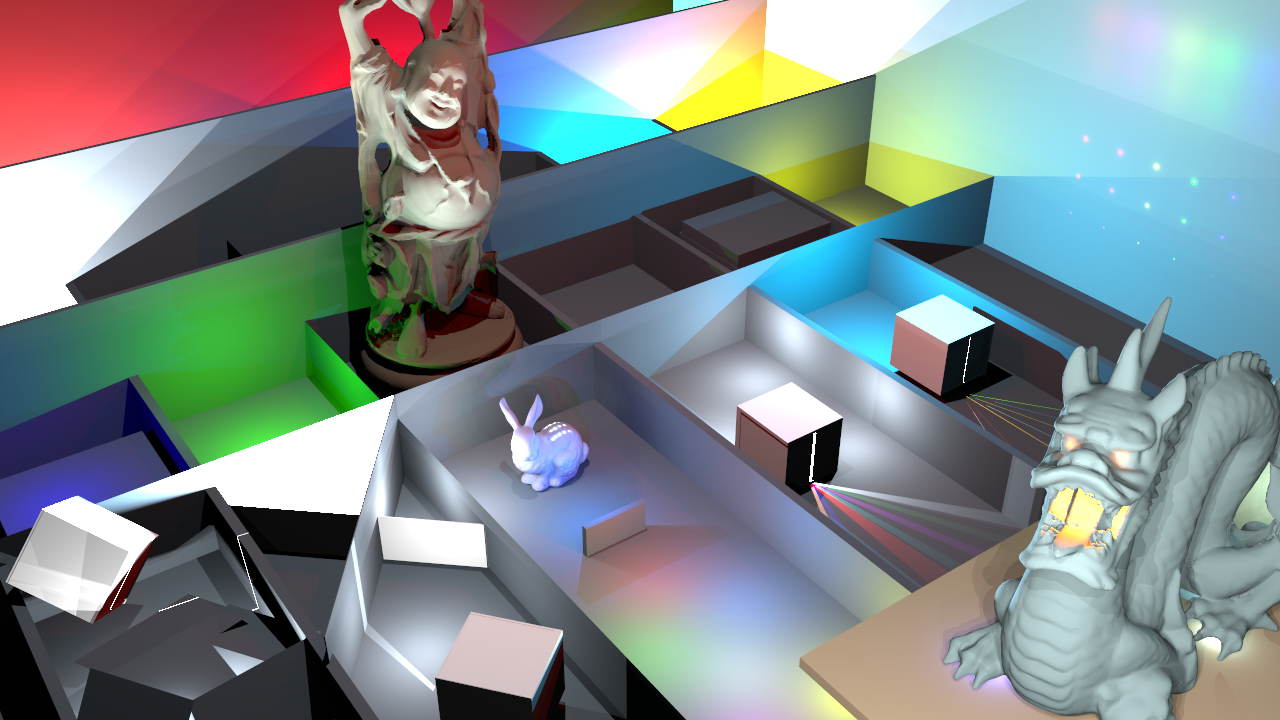
\includegraphics[width=1\textwidth]{figures/StanfordMuseum_ref.png}};
   
   \zoombox[magnification=0.8, color code=red]{0.85,0.3}
   \zoombox[magnification=1.5, color code=yellow]{0.334,0.78}
   
   \zoombox[magnification=2.3, color code=green]{0.767,0.47}
   \zoombox[magnification=1.4, color code=olive]{0.895,0.79}
   
   \zoombox[magnification=2, color code=brown]{0.285,0.32}
   \zoombox[magnification=1.3, color code=blue]{0.11,0.2}
   
   \zoombox[magnification=2, color code=cyan]{0.085,0.63}
   \zoombox[magnification=2, color code=pink]{0.6,0.68}

\end{tikzpicture}
\begin{tikzpicture}[overlay,remember picture]

\foreach \X in {1,...,\thezoombox}
   {\node[anchor=south,yshift=-13pt] at (zoombox-\X.south) 
   {\tiny (\X)};}
   \setcounter{zoombox}{0} 
\end{tikzpicture}

\caption{The reference image for \textit{Stanford-Museum} sampled with PBRTs directlighting integrator. Instead of NEE every light source is queried for any shading point. Max depth is one, thus no indirect illumination is present. All and more phenomenons from listing~\ref{li:problemcases} appear in this scene. Detailed descriptions and intentions of the zoomed areas are listed in~\ref{li:stanfordmuseum}.
}
\label{fig:stanfordmuseumref}
\end{figure}

We describe the most important problem cases we had in mind when designing the Stanford-Museum scene in figure~\ref{fig:stanfordmuseumref}, which is the reference image we calculate the MSE against. The scene contains 4058 light sources, all of whom are point light sources. We chose point light sources, because sampling a point on a area light source is not a concern of PNEE, thus reducing variance from other effects does discloses artifacts produced by our techniques more clearly. We also render the scene with a pathtracer with a max depth parameter of one, again, using the same argument, as depth introduces variance from the indirect lighting term of the pathtracer. Additionally, this makes rendering a nearly perfect reference image possible, by using PBRTs direct lighting integrator, which samples all point light sources for any intersection point. The reference image is rendered with 128 samples per pixel in 17 hours on our test machine. 

\begin{itemize}
    \item[(1)] The dragon is 20 times smaller than the Buddah but is very close to the camera and as such takes up almost the same screen space. Several low intensity point lights illuminate the dragon. The difference in size as well as light intensity constitute typical problem cases with LOD. Especially the illumination of the eyes is a rather extreme case, light source intensity is roughly 200.000 times less compared to the strongest light sources in the scene. Additionally, the left outline of the dragon is illuminated by various light sources from bellow in the scene, where the dragon takes up only an incredibly small solid angle and thus photons are very unlikely to hit the dragon.
    \item[(2)] The Buddah stands out of all cells and as such is illuminated by almost all visible light sources in this scene. This is particularly a problem for example with \textit{photontree}. There might be more light sources influencing a shading point, than the total number of nearest neighbors we collect. High geometric detail and blending of many light colors make the Buddah prone to fireflies.  All three Stanford models are also intended to add complexity for intersection tests to various parts of the scene. 
    \item[(3)] The box has a very tiny split from which is casts long range, very bright, very thin and high frequent light rays. Additionally, a lot of photons are stuck within the thin walled box, which highly complicates building good estimators with PNEE on the outside. Several more of this boxes with varying properties and surroundings are present in the scene. 
    \item[(4)] Similar to the Buddah this plane wall is illuminated by many light sources in the scene. Additionally, there is a matrix of point lights with varying brightness, distance and color. This variety has to be mapped to smooth transitions and high frequencies accordingly. Similar scenarios to this one do also appear in other parts of the scene, for example in front of the bunny, also with many smooth transitions, but where difficulties brought by global illumination are replaced with many local soft shadows. 
    \item[(5)] A cluster of roughly 1000 light sources. Only thin, non axis-aligned walls separates it from several distinct lightning scenarios. Very high exposure (unintentionally) breaks anti-aliasing. Most light sources influence the Buddah softly from bellow. 
    \item[(6)] Several non-axis aligned thin walls cover up a small cluster of light sources and cast thin, high frequent light rays in many directions. Especially the rays casted onto the scewed box, where photons from within the box, like mentioned in (3), do no good for our estimators, do constitute a tricky shading scenario in various manners.
    \item[(7)] Several strong light sources cast long range, smoothly fading, but sharp edged light rays. A similar scenario is present on the other side of the Buddah, where colors also blend together. The rays closely pass quite dark cells. Again, strong light sources behind a thin wall interfere with our photon collection algorithms.
    \item[(8)] A completely occluded light cluster with roughly 1000 light sources. In a real scene this might be a different room of a house for example. There are four such occluded clusters in the scene.
\label{li:stanfordmuseum}
\end{itemize}
\paragraph{Measure-one}




\paragraph{City}




\subsection{Techniques}

% which implementations will be compared

\subsection{Parameter Comparison}



%%%%%%%%%%%%%%%%%
\label{ch:ev:photontree}

%%%%%%%%%%%%%%%%%
\label{ch:ev:cdftree}

%%%%%%%%%%%%%%%%%%%%

\label{ch:ev:photonsampling}


%%%%%%%%%%%%%%%%%%%%%%%
\label{ch:ev:uniformfloor}

% which parameters did we try to configure. Which parameters turned out to be good and will be set as fixed?

\section{Equal time comparisons}

\section{Memory comparisons}

\section{Conclusions}

%% ==============
\chapter{Prospect}
\label{ch:Prospect}
%% ==============

We have demonstrated powerful results for PNEE in chapter~\ref{ch:Evaluation}. With speedups of around 50-100x in scenes with merely a couple thousand light sources, PNEE proves to be a great choice. A thousand light sources are well within the scope of typical real world production. For rather extreme cases with around a million light sources, results would be amplified. With hardly any drawbacks, we found no peril in using \textit{Cdfgrid} as a standard even for low complexity scenes. Direct comparison to very recent work from \textcite{Vevoda:2018:BOR} and \textcite{Estevez} would be highly interesting.

 We have already discussed some improvements and future work in section~\ref{sec:futhercons}. Mainly improvements for adaptive paramentrization are substantial for increasing the ease of use. Adding Multiple Importance Sampling with adaptive importance weights might also be a valuable addition in the future. Exploring the possibility to extend \textit{Cdfgrid} for adaptive LOD with an Octree was discussed in section~\ref{ch:octree}. Improvements on importance sampling the initial photon distribution, as discussed in section~\ref{ch:photonimportancesample}, might also be worthwhile to explore. We examined several interpolation and approximation schemes in section~\ref{ch:interpolation}, but there is still plenty of research that can be done. It has been an exciting task \unsure{Ist das zu umgangssprachlich hier schon?} to adapt and optimize traditional interpolation schemes to CDFs and our specific needs. 

Our construction of interpolated CDFs (section~\ref{sec:intcdf}) and sparse CDFs (section~\ref{sec:sparse}) have proven to be effective additions and may be of value for other research, too. The general idea of PNEE can be ported to other ray tracers like MLT or BDPT\unsure{Nicht ganz sicher}. Also, photon mapping can be extended with PNEE, essentially for free, since photons are shot and stored anyhow. In an interactive context, PNEE might be explored but might be tricky due to the preprocess. In the case where only the camera will be moved, PNEE is particularly suited, as the photons and data structures can be reused. Lastly, the idea of PNEE is potentially extendable to path guiding (see e.g. \parencite{DBLP:journals/cgf/MullerGN17}), where NEE can be regarded as just the last step in a series of subproblems.

\unsure{Ist das Kapitel ausreichend vom Umfang?}

\newpage
\section*{Acronyms}

\begin{acronym}[ECU]


\acro{AHC}[AHC]{Agglomerative Hierarchical Clustering}


\acro{BSDF}[BSDF]{Bidirectional scattering distribution function}
\acro{BRDF}[BRDF]{Bidirectional reflectance distribution function}

\acro{CDF}[CDF]{Cumulative distribution function}

\acro{IS}[IS]{Importance Sampling}

\acro{LOD}[LOD]{Level of detail}

\acro{MIS}[MIS]{Multiple Importance Sampling}
\acro{MSE}[MSE]{Mean Squared Error}

\acro{NEE}[NEE]{Next Event Estimation}
\acro{NN}[NN]{Nearest Neighbour(s)}

\acro{PBRT}[PBRT]{Physically Based Rendering}
\acro{PDF}[PDF]{Probability distribution function}
\acro{PNEE}[PNEE]{Photon-based Next Event Estimation}


\end{acronym}


\appendix 
%\addcontentsline{toc}{chapter}{APPENDICES}

\chapter{Images}

\begin{figure}
    \centering
    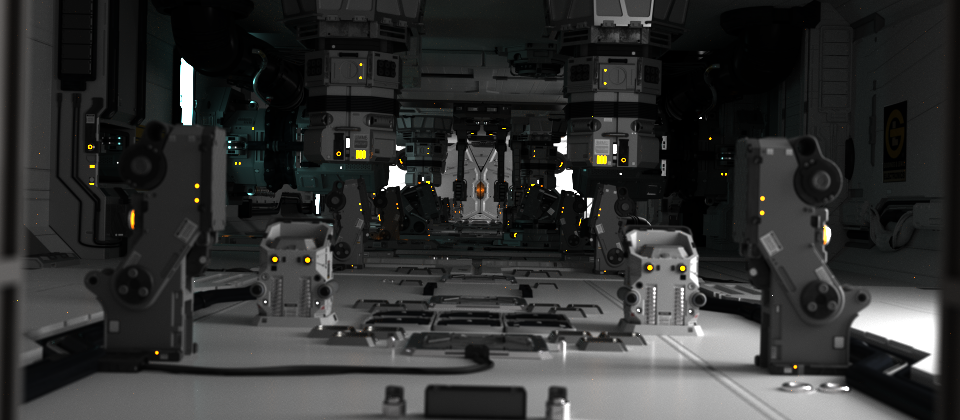
\includegraphics[width=1\textwidth]{figures/References/frame25_spat_REF_ps12288_t43568_47001.png}
    \caption{Zero-Day reference image}
    \label{fig:zdref}
\end{figure}

\begin{figure}
    \centering
    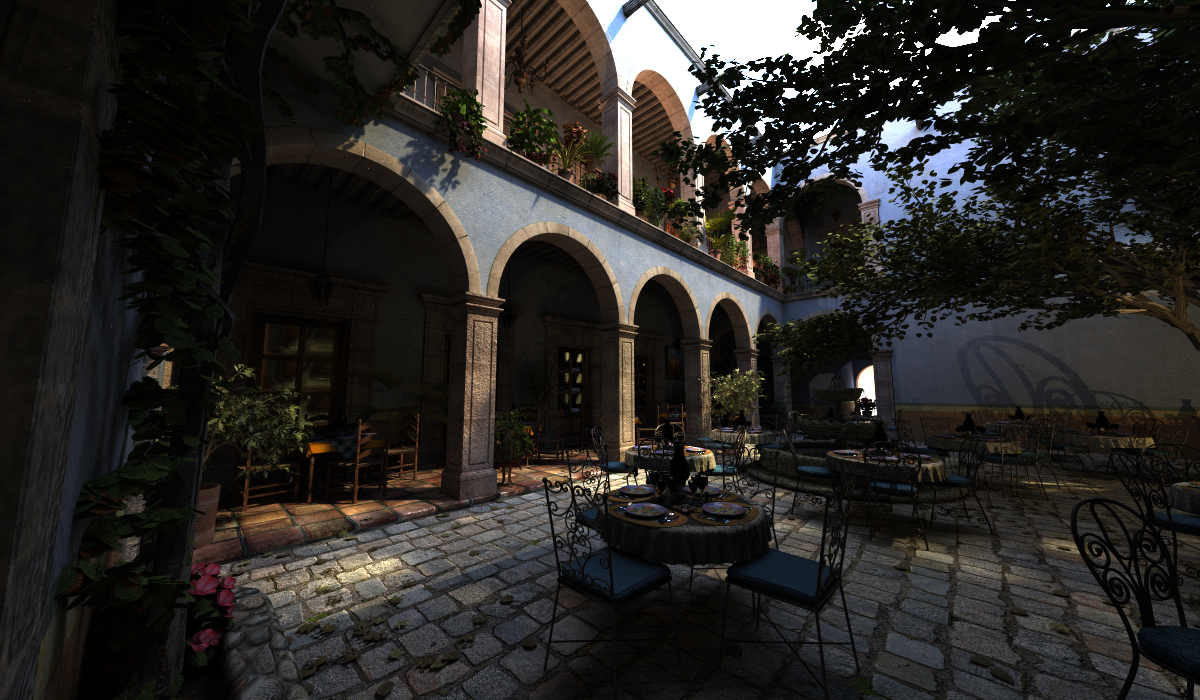
\includegraphics[width=1\textwidth]{figures/References/sanmiguel_cam25_REF_spat_ps8192_t59288_71697.png}
    \caption{San Miguel reference image}
    \label{fig:smigref}
\end{figure}


%% --------------------
%% |   Bibliography   |
%% --------------------
\cleardoublepage
\phantomsection
\addcontentsline{toc}{chapter}{\bibname}

%\iflanguage{english}
%{\bibliographystyle{IEEEtranSA}}	% english style
%{\bibliographystyle{babalpha-fl}}	% german style
%\bibliographystyle{apalike}

												  
% Use IEEEtran for numeric references
%\bibliographystyle{IEEEtranSA})

\printbibliography
\Erklaerung
\end{document}
